\documentclass[tikz,border=5pt]{standalone}
\usepackage{tikz}
\usepackage{lmodern}
\usetikzlibrary{shapes,arrows,positioning,calc,fit}

\begin{document}
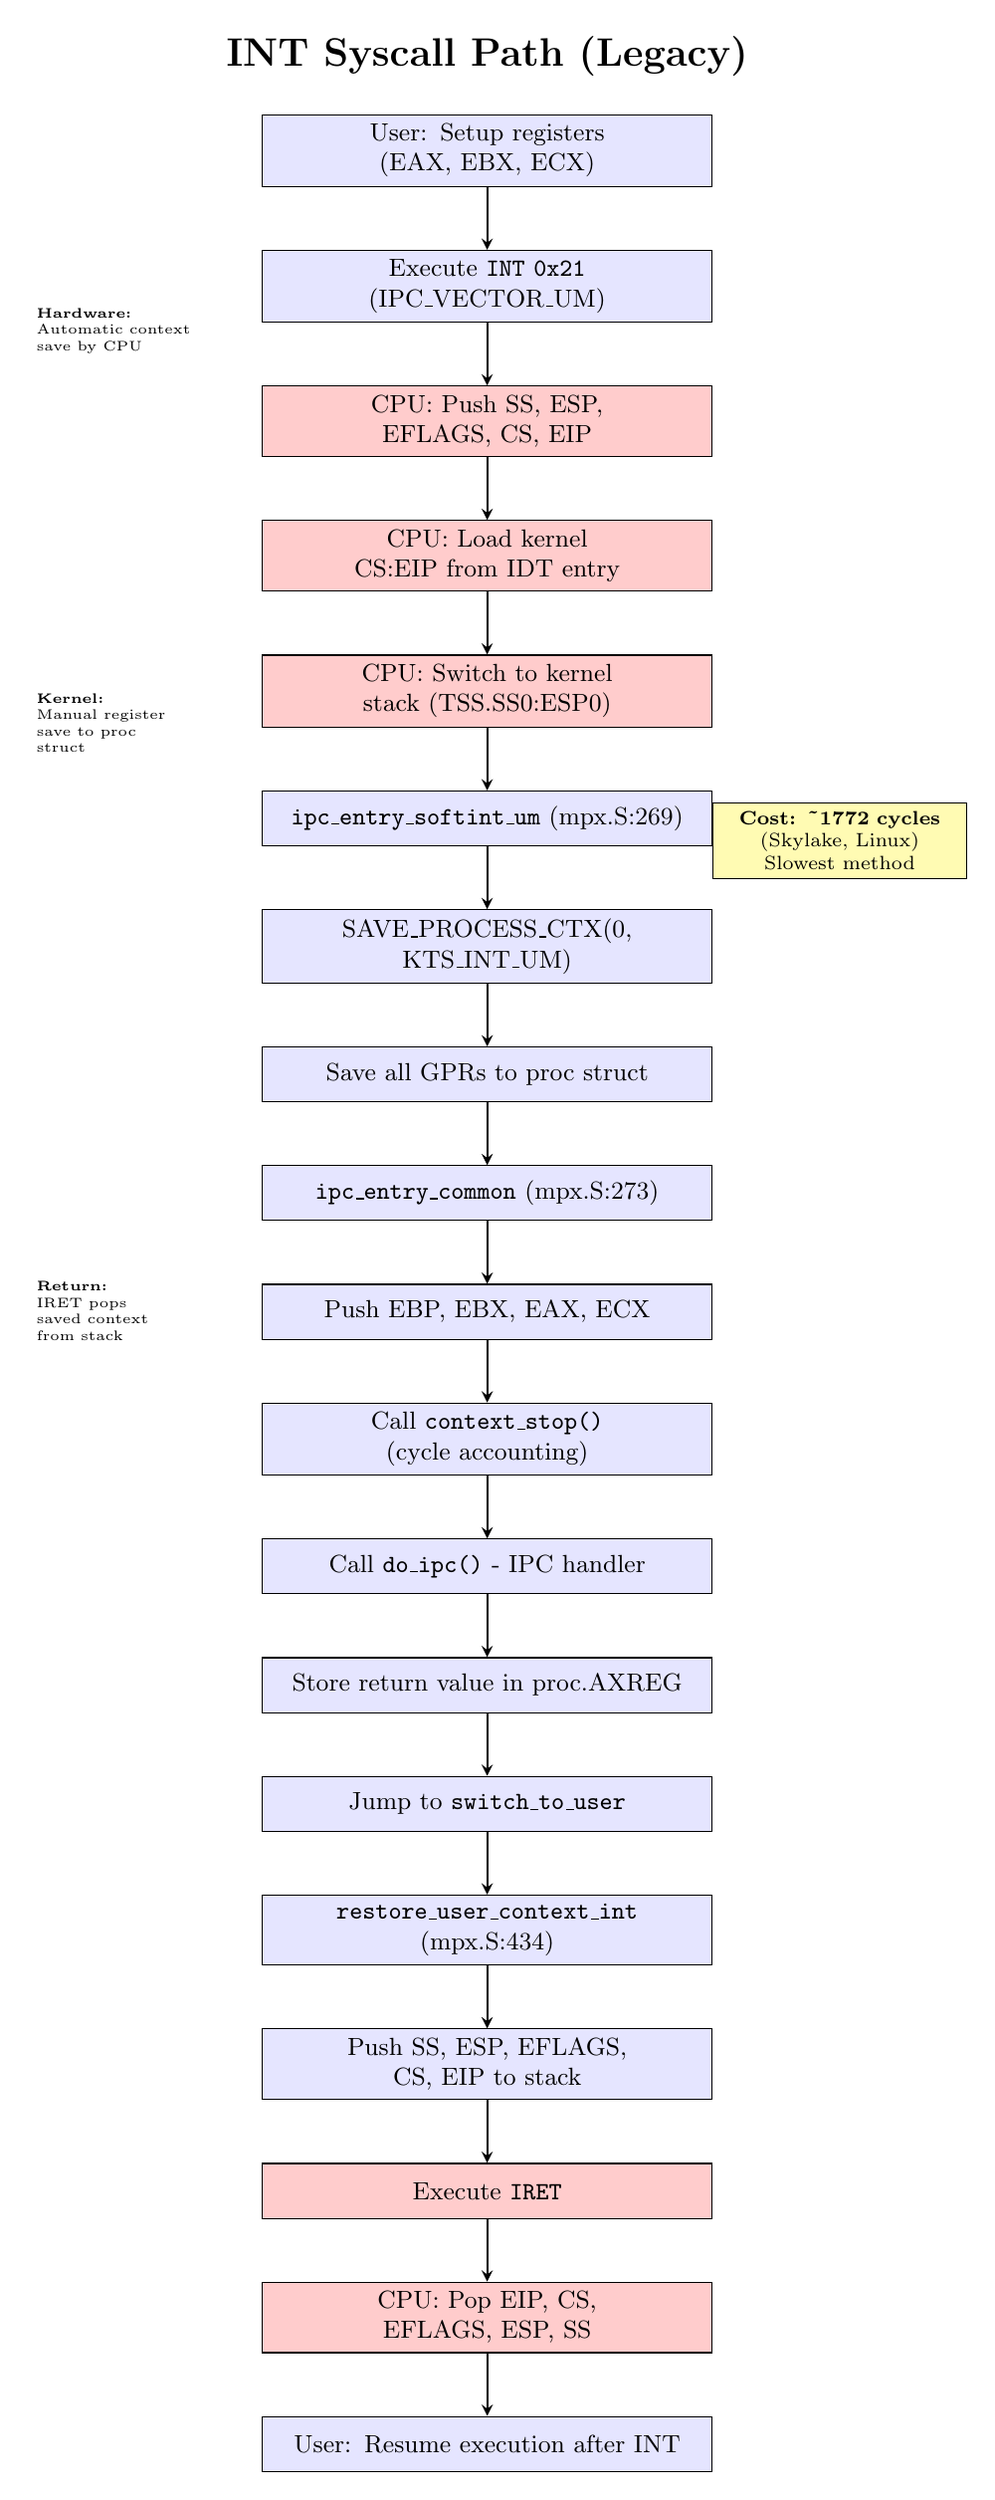
\begin{tikzpicture}[
    node distance=0.8cm,
    box/.style={rectangle, draw, fill=blue!10, text width=5.5cm, align=center, minimum height=0.7cm, font=\small},
    hw/.style={rectangle, draw, fill=red!20, text width=5.5cm, align=center, minimum height=0.7cm, font=\small},
    arrow/.style={->,>=stealth,thick}
]

% Title
\node[font=\Large\bfseries] at (0,0) {INT Syscall Path (Legacy)};

% User space
\node[box] (user1) at (0,-1.2) {User: Setup registers (EAX, EBX, ECX)};
\node[box] (user2) [below=of user1] {Execute \texttt{INT 0x21} (IPC\_VECTOR\_UM)};

% Hardware actions
\node[hw] (hw1) [below=of user2] {CPU: Push SS, ESP, EFLAGS, CS, EIP};
\node[hw] (hw2) [below=of hw1] {CPU: Load kernel CS:EIP from IDT entry};
\node[hw] (hw3) [below=of hw2] {CPU: Switch to kernel stack (TSS.SS0:ESP0)};

% Kernel entry
\node[box] (kern1) [below=of hw3] {\texttt{ipc\_entry\_softint\_um} (mpx.S:269)};
\node[box] (kern2) [below=of kern1] {SAVE\_PROCESS\_CTX(0, KTS\_INT\_UM)};
\node[box] (kern3) [below=of kern2] {Save all GPRs to proc struct};
\node[box] (kern4) [below=of kern3] {\texttt{ipc\_entry\_common} (mpx.S:273)};
\node[box] (kern5) [below=of kern4] {Push EBP, EBX, EAX, ECX};
\node[box] (kern6) [below=of kern5] {Call \texttt{context\_stop()} (cycle accounting)};
\node[box] (kern7) [below=of kern6] {Call \texttt{do\_ipc()} - IPC handler};

% Return path
\node[box] (ret1) [below=of kern7] {Store return value in proc.AXREG};
\node[box] (ret2) [below=of ret1] {Jump to \texttt{switch\_to\_user}};
\node[box] (ret3) [below=of ret2] {\texttt{restore\_user\_context\_int} (mpx.S:434)};
\node[box] (ret4) [below=of ret3] {Push SS, ESP, EFLAGS, CS, EIP to stack};
\node[hw] (hw4) [below=of ret4] {Execute \texttt{IRET}};
\node[hw] (hw5) [below=of hw4] {CPU: Pop EIP, CS, EFLAGS, ESP, SS};
\node[box] (user3) [below=of hw5] {User: Resume execution after INT};

% Arrows
\foreach \i/\j in {user1/user2, user2/hw1, hw1/hw2, hw2/hw3, hw3/kern1, kern1/kern2, kern2/kern3, kern3/kern4, kern4/kern5, kern5/kern6, kern6/kern7, kern7/ret1, ret1/ret2, ret2/ret3, ret3/ret4, ret4/hw4, hw4/hw5, hw5/user3} {
    \draw[arrow] (\i) -- (\j);
}

% Side annotations
\node[font=\tiny, text width=2.5cm, align=left] at (-4.5,-3.5) {
    \textbf{Hardware:}\\
    Automatic context\\
    save by CPU
};

\node[font=\tiny, text width=2.5cm, align=left] at (-4.5,-8.5) {
    \textbf{Kernel:}\\
    Manual register\\
    save to proc\\
    struct
};

\node[font=\tiny, text width=2.5cm, align=left] at (-4.5,-16) {
    \textbf{Return:}\\
    IRET pops\\
    saved context\\
    from stack
};

% Cycle cost annotation
\node[font=\scriptsize, fill=yellow!30, draw, text width=3cm, align=center] at (4.5,-10) {
    \textbf{Cost: \textasciitilde1772 cycles}\\
    (Skylake, Linux)\\
    Slowest method
};

\end{tikzpicture}
\end{document}
